\documentclass{article}

\usepackage[utf8]{inputenc}

\usepackage{amsmath, bm}
\usepackage{graphicx}
\usepackage{amssymb}
\usepackage{float}
\usepackage{caption}
\usepackage{subcaption}
\usepackage{hyperref}
\usepackage{tikz}
\usepackage{layout}

\usepackage[margin=1in]{geometry}
\usepackage{listings}
\usepackage{xcolor}
\usepackage{color, colortbl}
\usepackage{textgreek}
\usepackage{mathrsfs}
\usepackage{savetrees}
\usepackage{booktabs}

\usepackage{titlesec}

\titleformat{\subsubsection}
  {\normalfont\selectfont}{\thesubsubsection}{1em}{}

\usetikzlibrary{calc}
\usetikzlibrary{angles,quotes} % for pic
\usetikzlibrary{patterns,snakes}
\usetikzlibrary{arrows}
\tikzset{>=latex} % for LaTeX arrow head

\setlength{\parskip}{\baselineskip}%
\setlength{\parindent}{0pt}%
\linespread{0.9}


\definecolor{codegreen}{rgb}{0,0.6,0}
\definecolor{codegray}{rgb}{0.5,0.5,0.5}
\definecolor{codepurple}{rgb}{0.58,0,0.82}
\definecolor{backcolour}{rgb}{0.95,0.95,0.92}

\lstdefinestyle{mystyle}{
    backgroundcolor=\color{backcolour},   
    commentstyle=\color{codegreen},
    keywordstyle=\color{magenta},
    numberstyle=\tiny\color{codegray},
    stringstyle=\color{codepurple},
    basicstyle=\ttfamily\footnotesize,
    breakatwhitespace=false,         
    breaklines=true,                 
    captionpos=b,                    
    keepspaces=true,                 
    numbers=left,                    
    numbersep=5pt,                  
    showspaces=false,                
    showstringspaces=false,
    showtabs=false,                  
    tabsize=2
}

\lstset{style=mystyle}



\begin{document}

\title{}
\author{lwp26}
\date{January 2025}
\maketitle

\section{Results}

\subsection{Longitudinal Static Stability}

\begin{table}[H]
    \centering
    \begin{tabular}{lrrr}
        \toprule
         & Fuel Mass (kg) & CG position relative to MAC (-) & Total Mass (kg) \\
        \midrule
        A & 1873.300 & 33.087 & 12514.300 \\
        B & 1538.500 & 24.807 & 12271.500 \\
        \bottomrule
        \end{tabular}
\end{table}

\begin{table}[H]
    \centering
    \begin{tabular}{lllll}
        \toprule
         Group A & Ve kt EAS & Elev deflection deg & Elev tab angle deg & Weight Coefficient - \\
        \midrule
        & 181.250 & 0.248 & 0.321 & 0.553 \\
        & 170.781 & -0.049 & 0.504 & 0.623 \\
        & 160.484 & -0.431 & 0.735 & 0.705 \\
        & 190.594 & 0.786 & 0.001 & 0.500 \\
        & 199.109 & 0.997 & -0.205 & 0.458 \\
        \bottomrule
        \end{tabular}
    \end{table}
\begin{table}[H]
    \centering        
    \begin{tabular}{lllll}
        \toprule
         Group B & Ve kt EAS & Elev deflection deg & Elev tab angle deg & Weight Coefficient - \\
        \midrule
         & 180.422 & -1.474 & 1.081 & 0.547 \\
         & 170 & -2.078 & 1.448 & 0.616 \\
         & 160.297 & -2.731 & 1.837 & 0.693 \\
         & 190.250 & -1.054 & 0.753 & 0.492 \\
         & 200.844 & -0.536 & 0.420 & 0.441 \\
        \bottomrule
        \end{tabular}
\end{table}

\subsubsection{Stick fixed neutral point}

\begin{figure}[H]
    \centering
    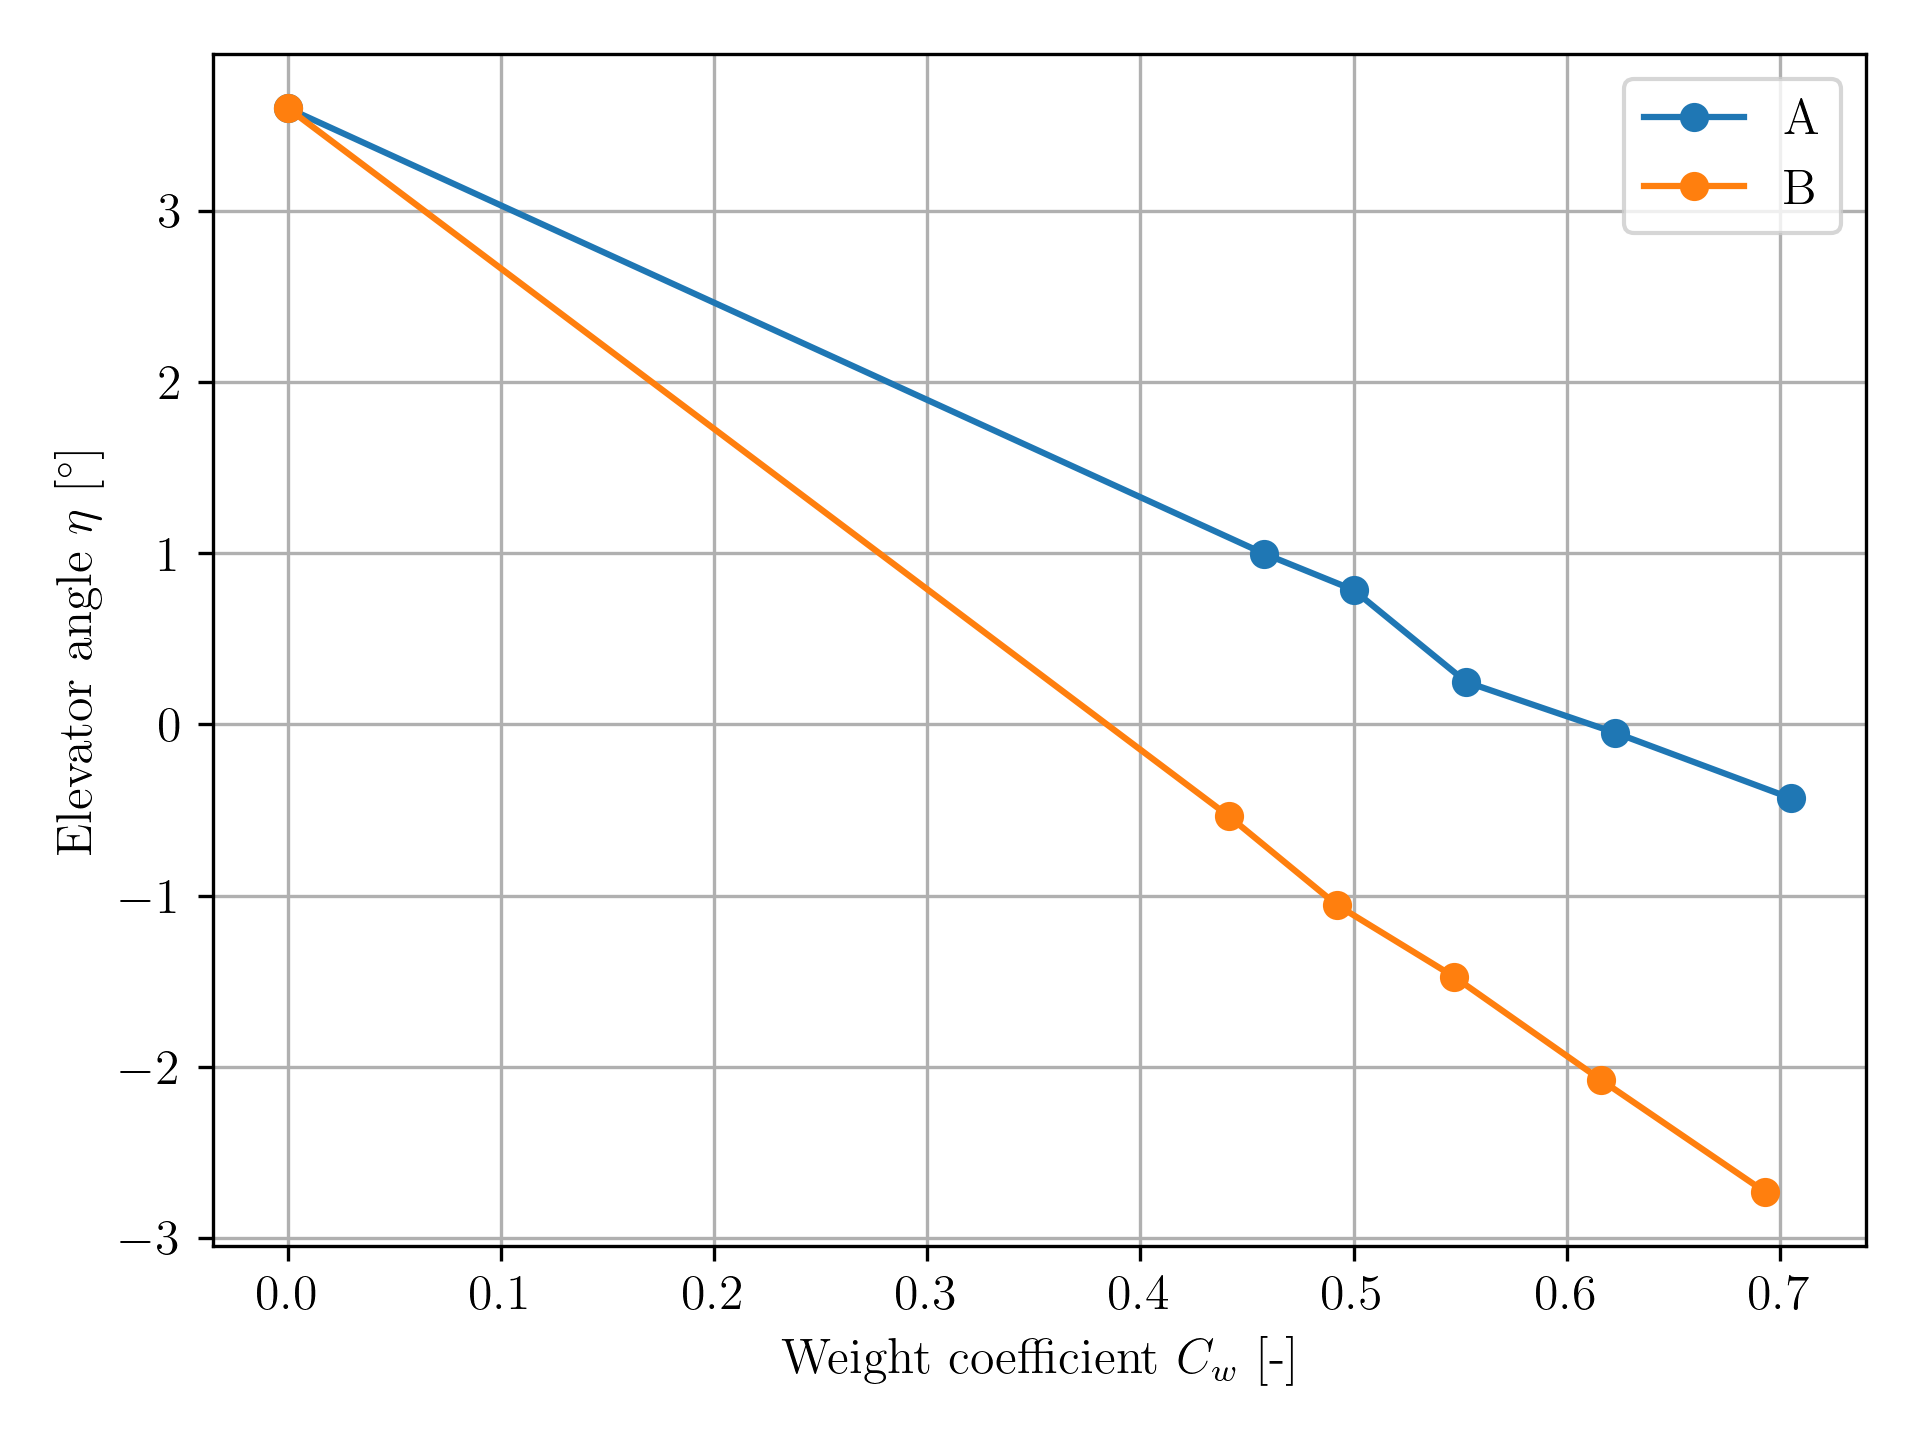
\includegraphics[width=0.8\textwidth]{Longitudinal_Static_Stability_1.png}
    \caption{}
    \label{fig:Longitudinal_Static_Stability_1}
\end{figure}
\begin{figure}[H]
    \centering
    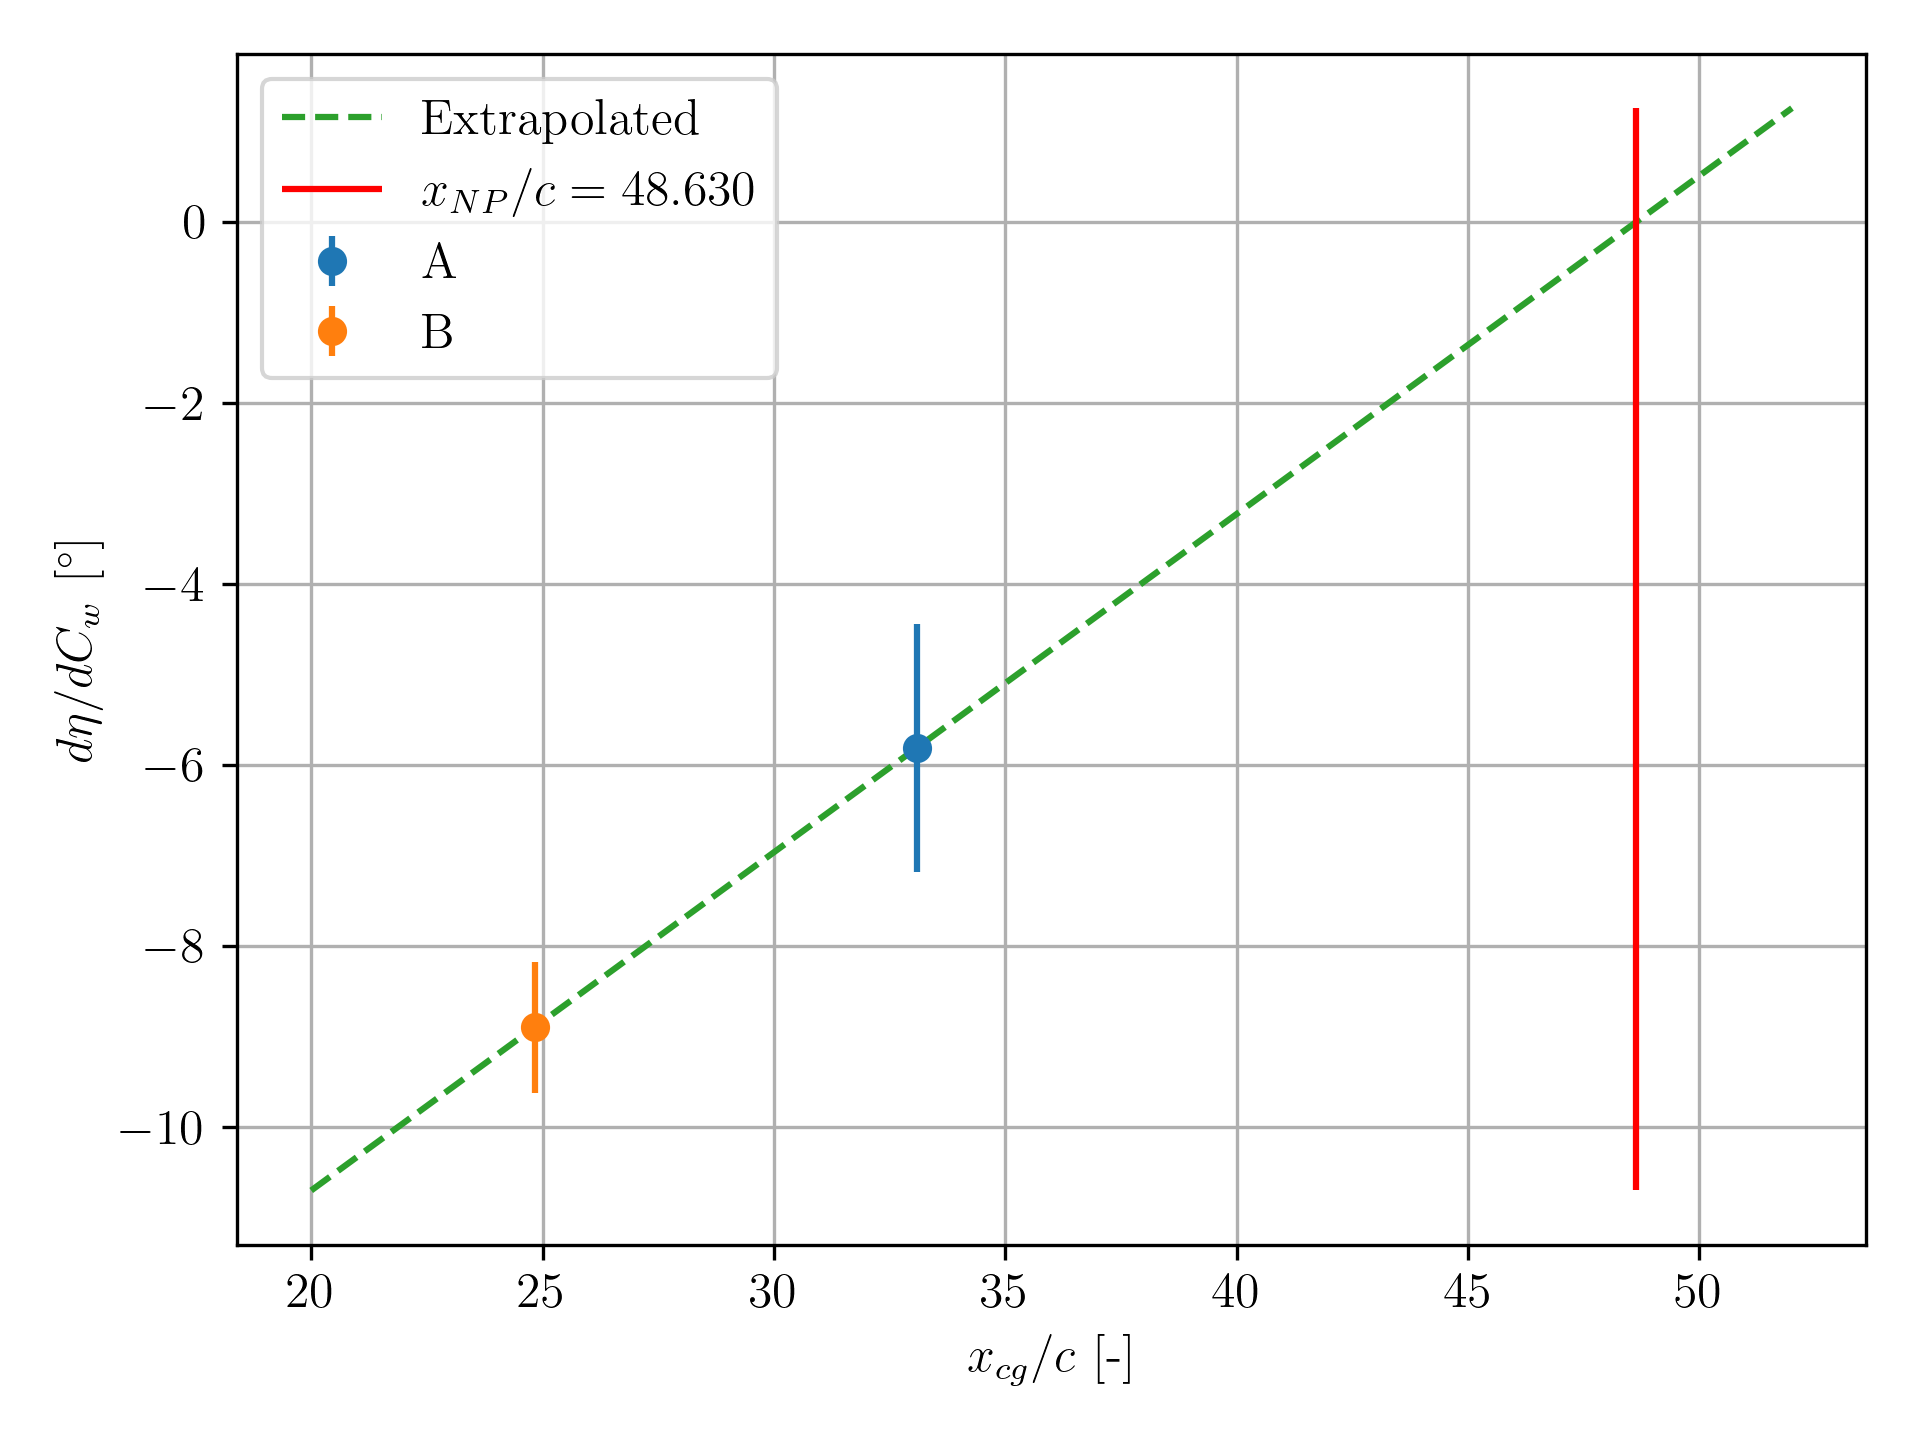
\includegraphics[width=0.8\textwidth]{Longitudinal_Static_Stability_2.png}
    \caption{}
    \label{fig:Longitudinal_Static_Stability_2}
\end{figure}

\subsubsection{Stick free neutral point}
\begin{figure}[H]
    \centering
    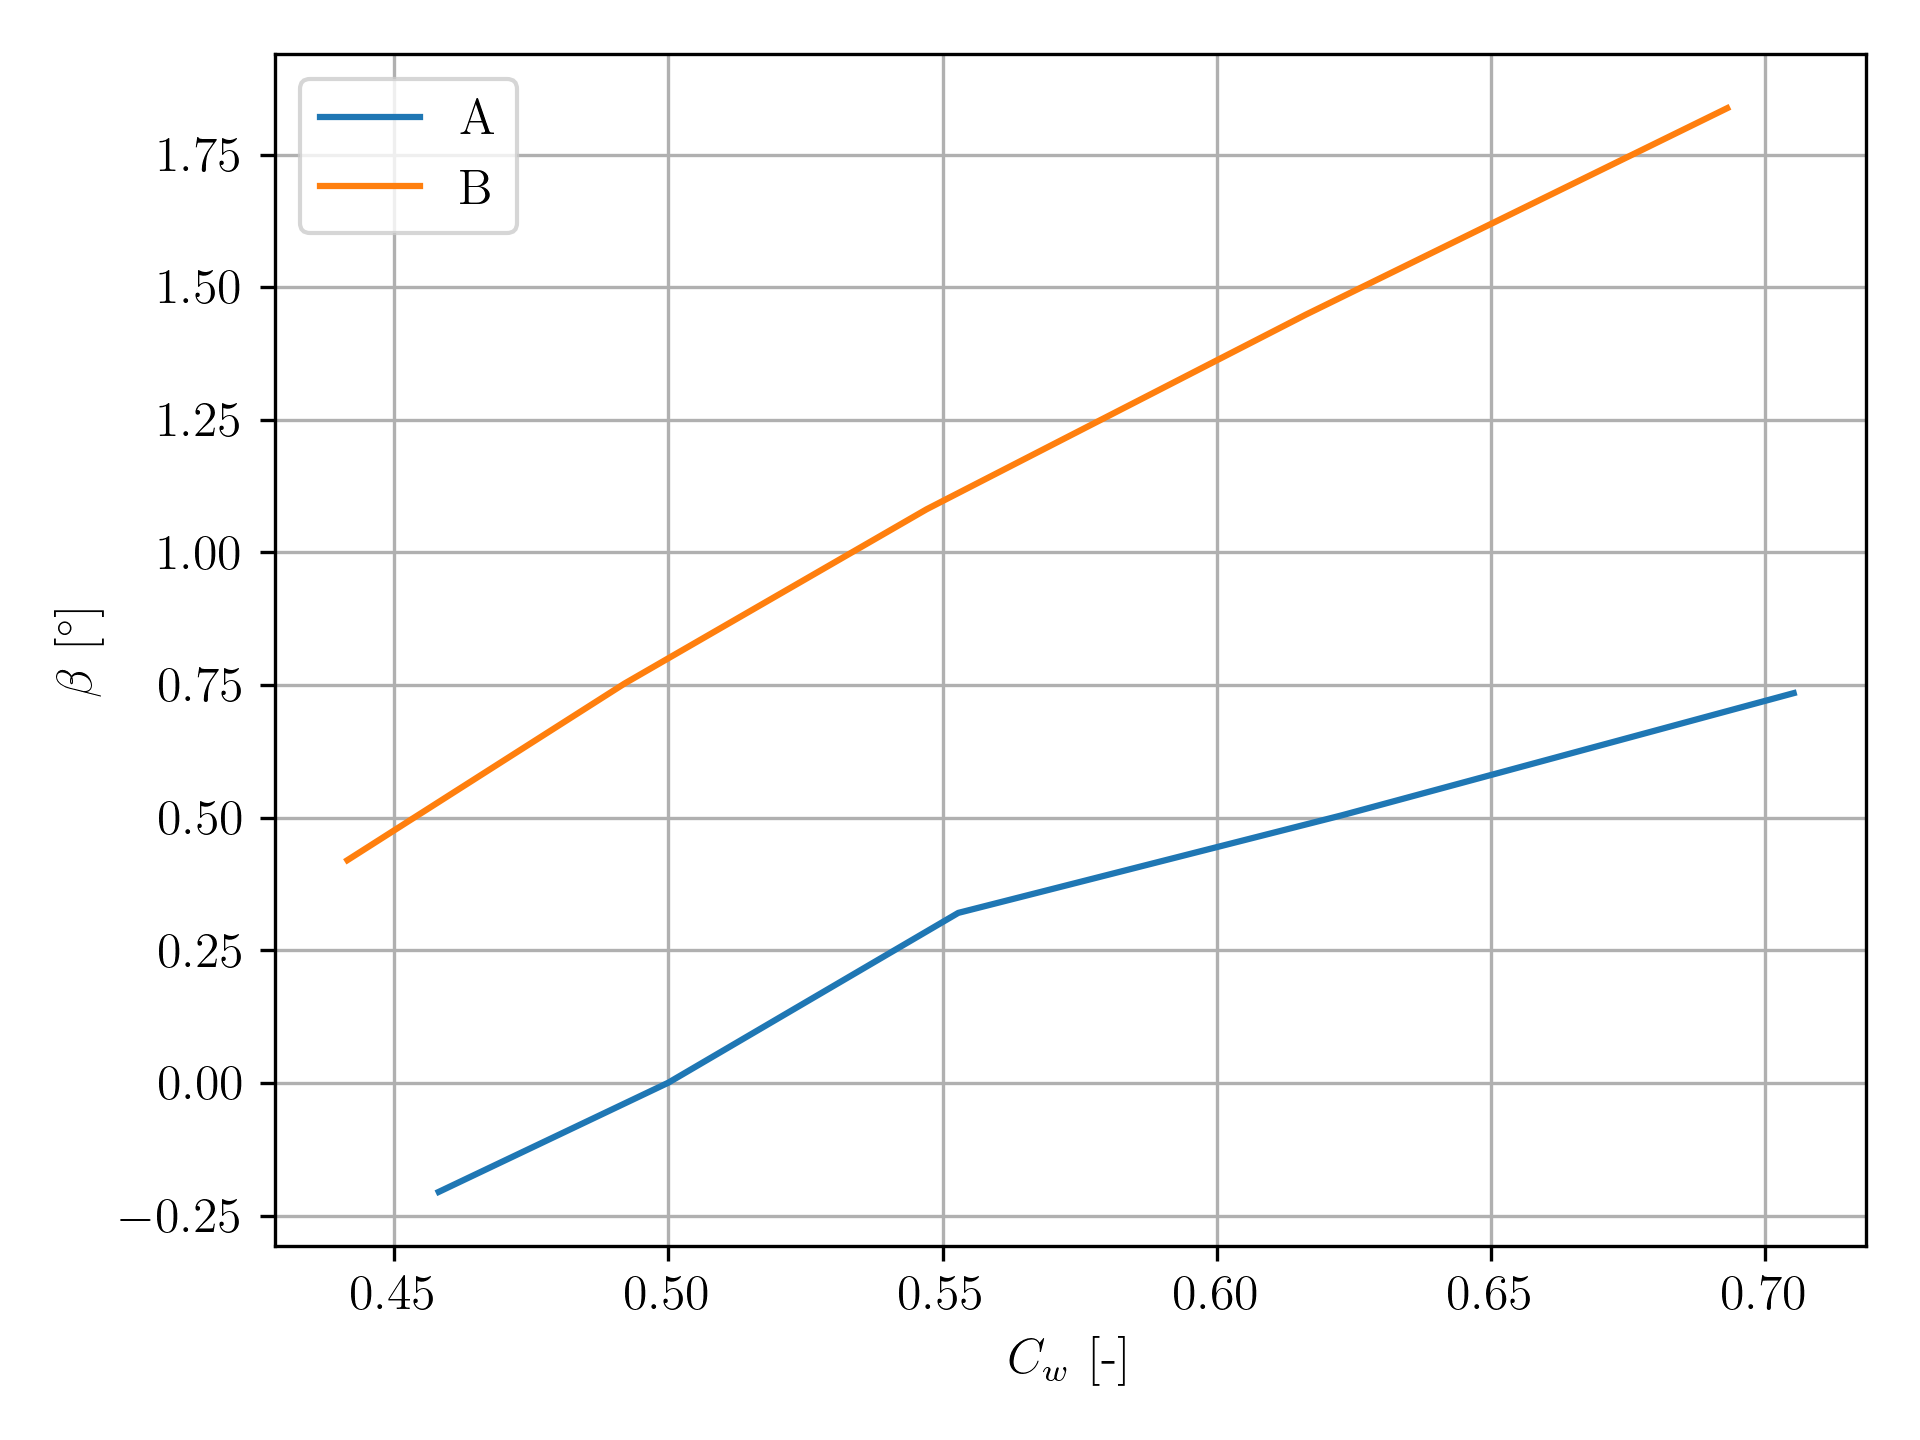
\includegraphics[width=0.8\textwidth]{Longitudinal_Static_Stability_3.png}
    \caption{}
    \label{fig:Longitudinal_Static_Stability_3}
\end{figure}
\begin{figure}[H]
    \centering
    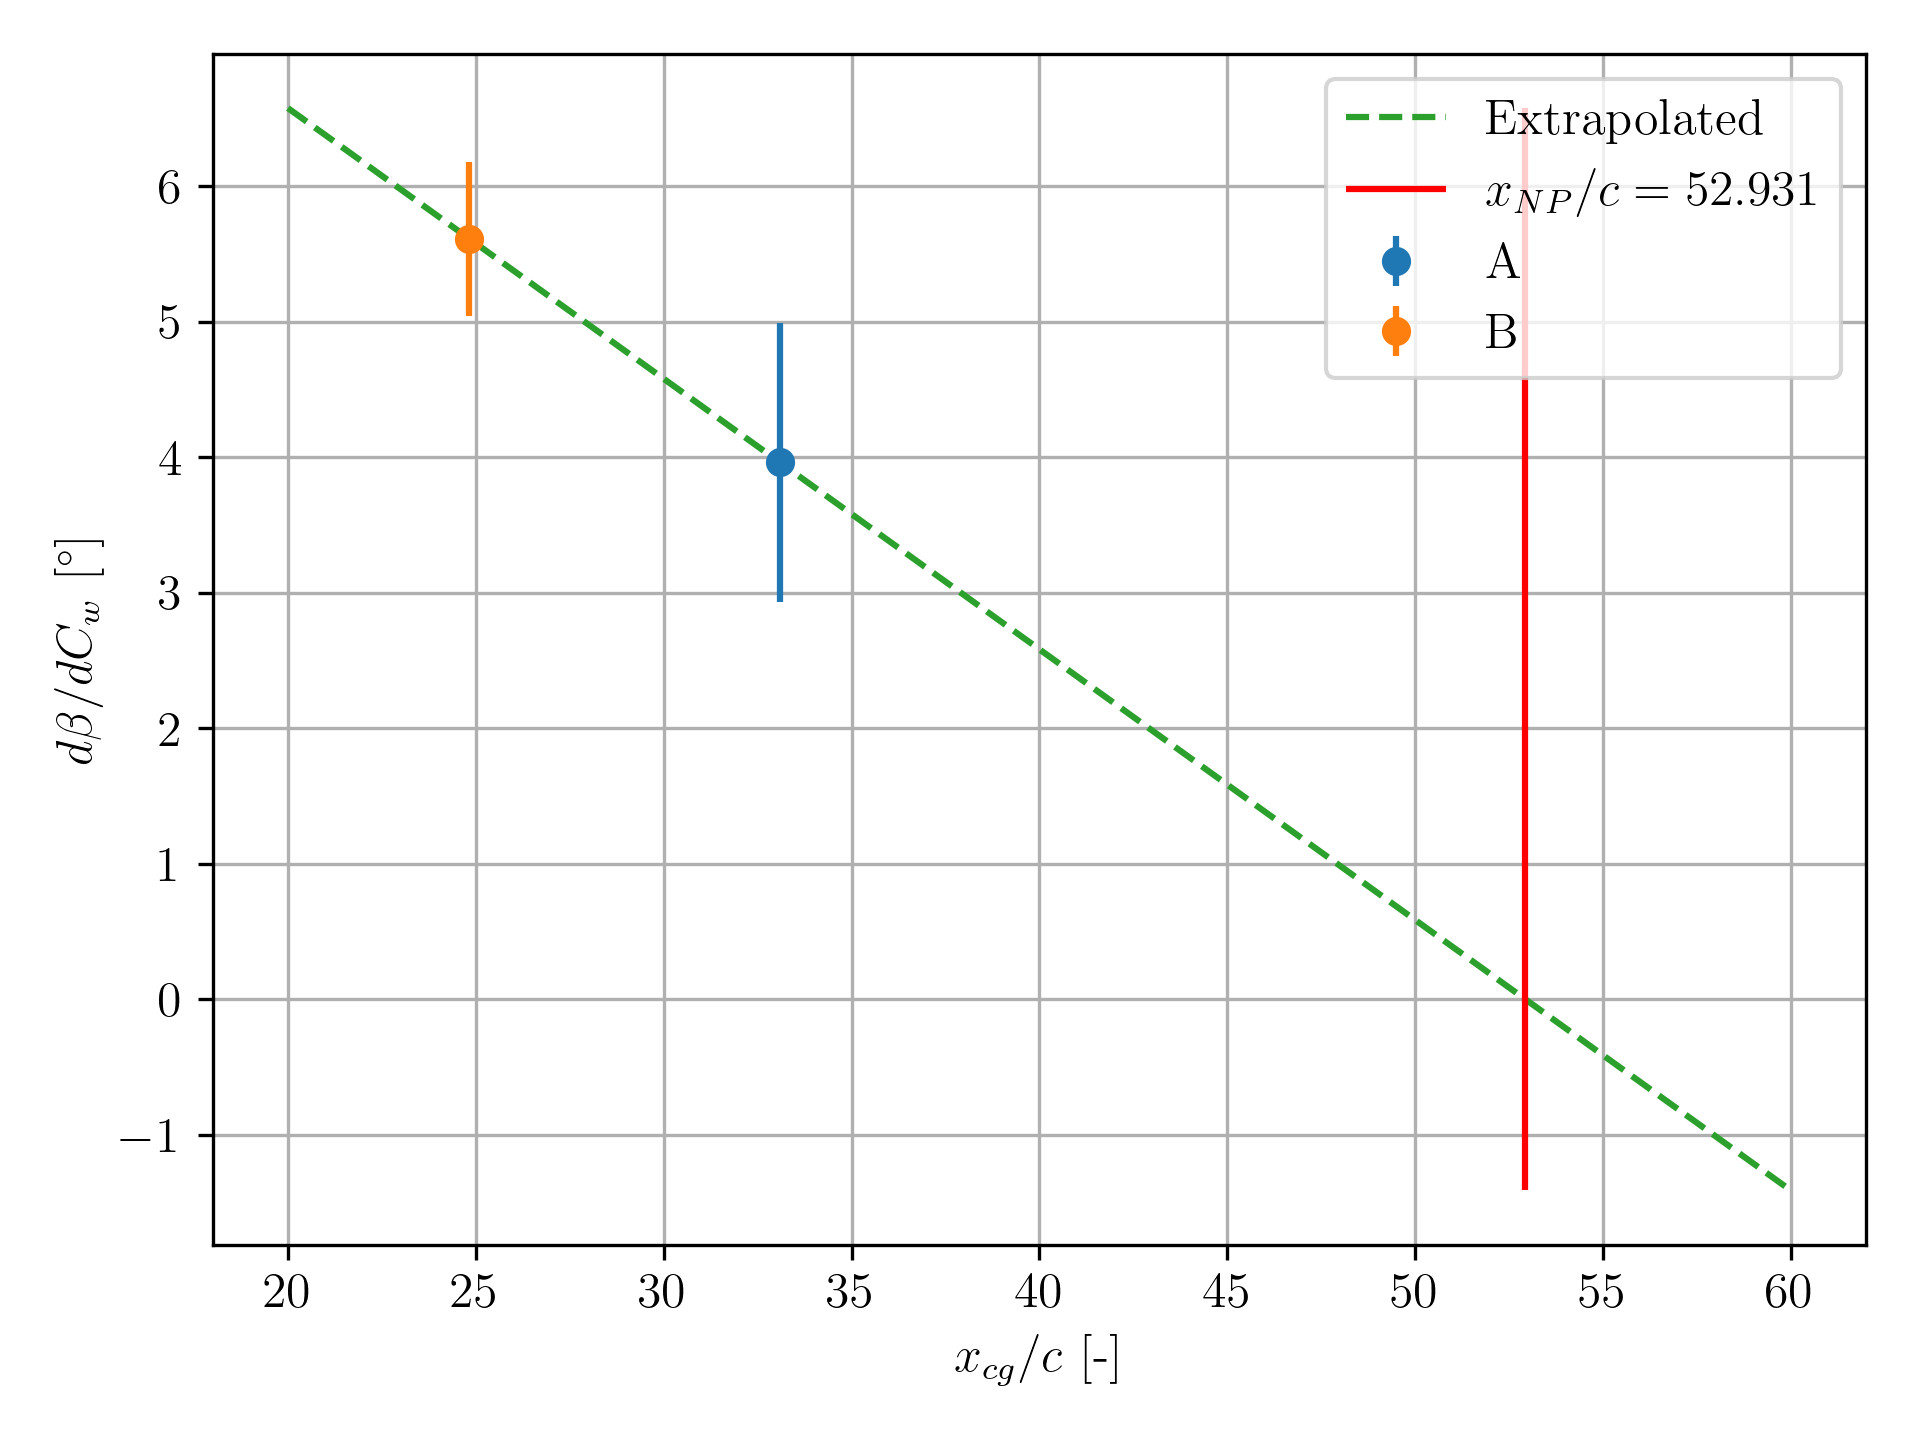
\includegraphics[width=0.8\textwidth]{Longitudinal_Static_Stability_4.png}
    \caption{}
    \label{fig:Longitudinal_Static_Stability_4}
\end{figure}

\subsection{Manoeuvre Stability}

\begin{table}[H]
    \centering
    \begin{tabular}{lrrr}
        \toprule
         & Fuel Mass (kg) & CG position relative to MAC (-) & Total Mass (kg) \\
        \midrule
        A & 1873.300 & 33.087 & 12514.300 \\
        B & 1538.500 & 24.807 & 12271.500 \\
        \bottomrule
        \end{tabular}
\end{table}

\begin{table}[H]
    \centering
    \begin{tabular}{lllll}
        \toprule
        Group A & Elev deflection deg & Stick force N & (n+1)g & Normal acceleration g \\
        \midrule
        & 0.203 & -65.302 & 1.044 & 0.044 \\
        & -0.681 & -16.824 & 1.122 & 0.122 \\
        & -1.187 & 23.435 & 1.192 & 0.192 \\
        & -2.981 & 146.032 & 1.434 & 0.434 \\
        & -5.052 & 245.931 & 1.950 & 0.950 \\
        \bottomrule
        \end{tabular}
\end{table}

\begin{table}[H]
    \centering
        \begin{tabular}{lllll}
        \toprule
        Group B & Elev deflection deg & Stick force N & (n+1)g & Normal acceleration g \\
        \midrule
        & -1.553 & 32.742 & 1.001 & 0.001 \\
        & -2.766 & 109.857 & 1.176 & 0.176 \\
        & -3.668 & 153.774 & 1.237 & 0.237 \\
        & -5.797 & 302.100 & 1.675 & 0.675 \\
        & -7.347 & 408.260 & 1.970 & 0.970 \\
        \bottomrule
        \end{tabular}
\end{table}

\subsubsection{Stick fixed manoeuvre point}
\begin{figure}[H]
    \centering
    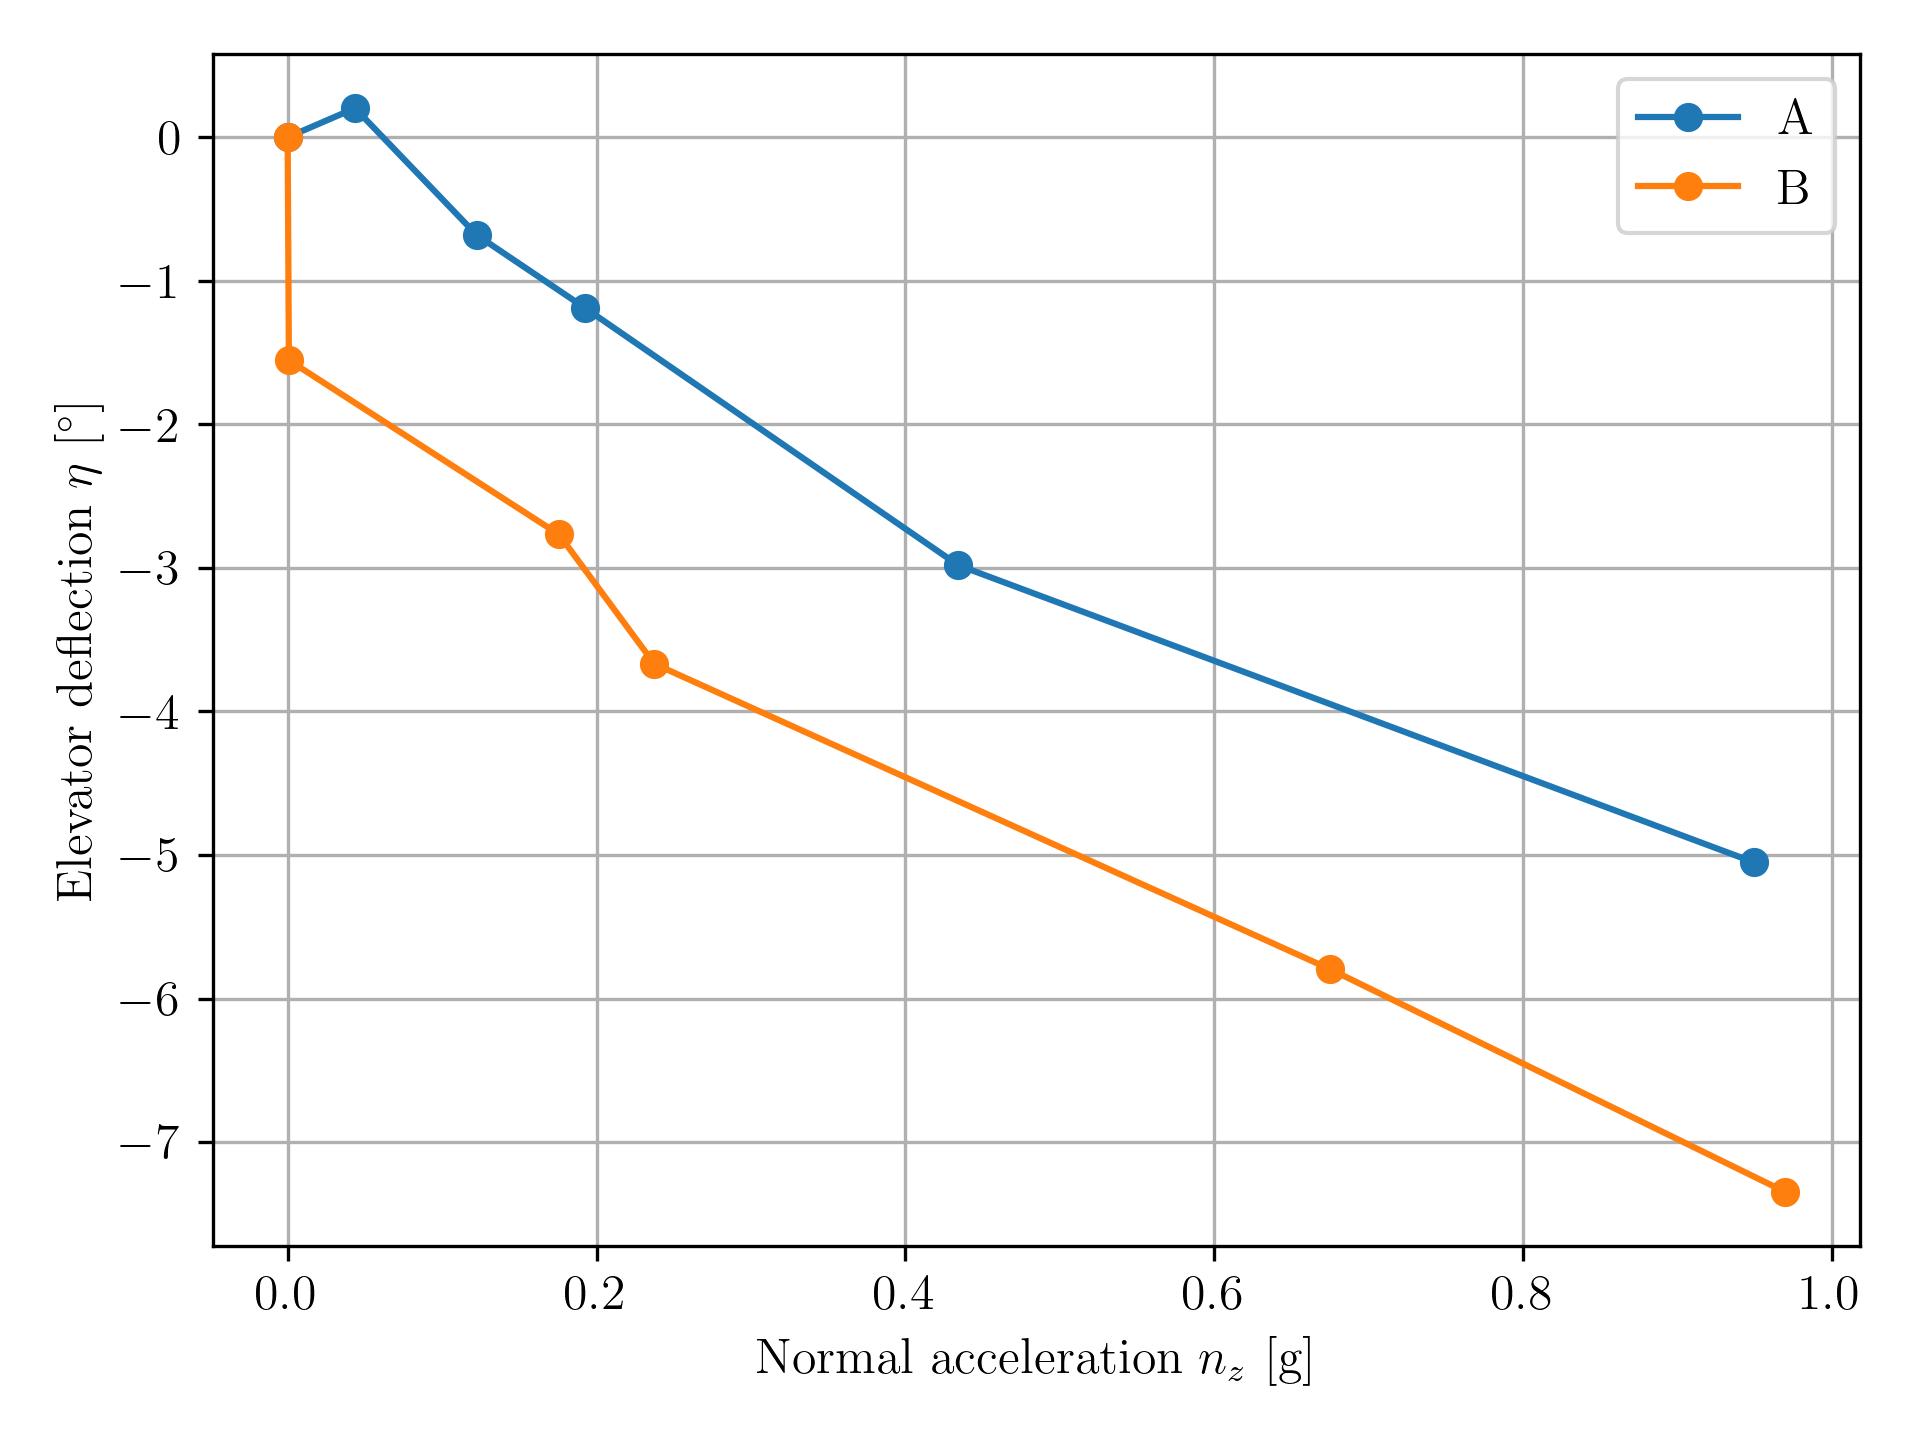
\includegraphics[width=0.8\textwidth]{Manoeuvre_Stability_1.png}
    \caption{}
    \label{fig:Manoeuvre_Stability_1}
\end{figure}
\begin{figure}[H]
    \centering
    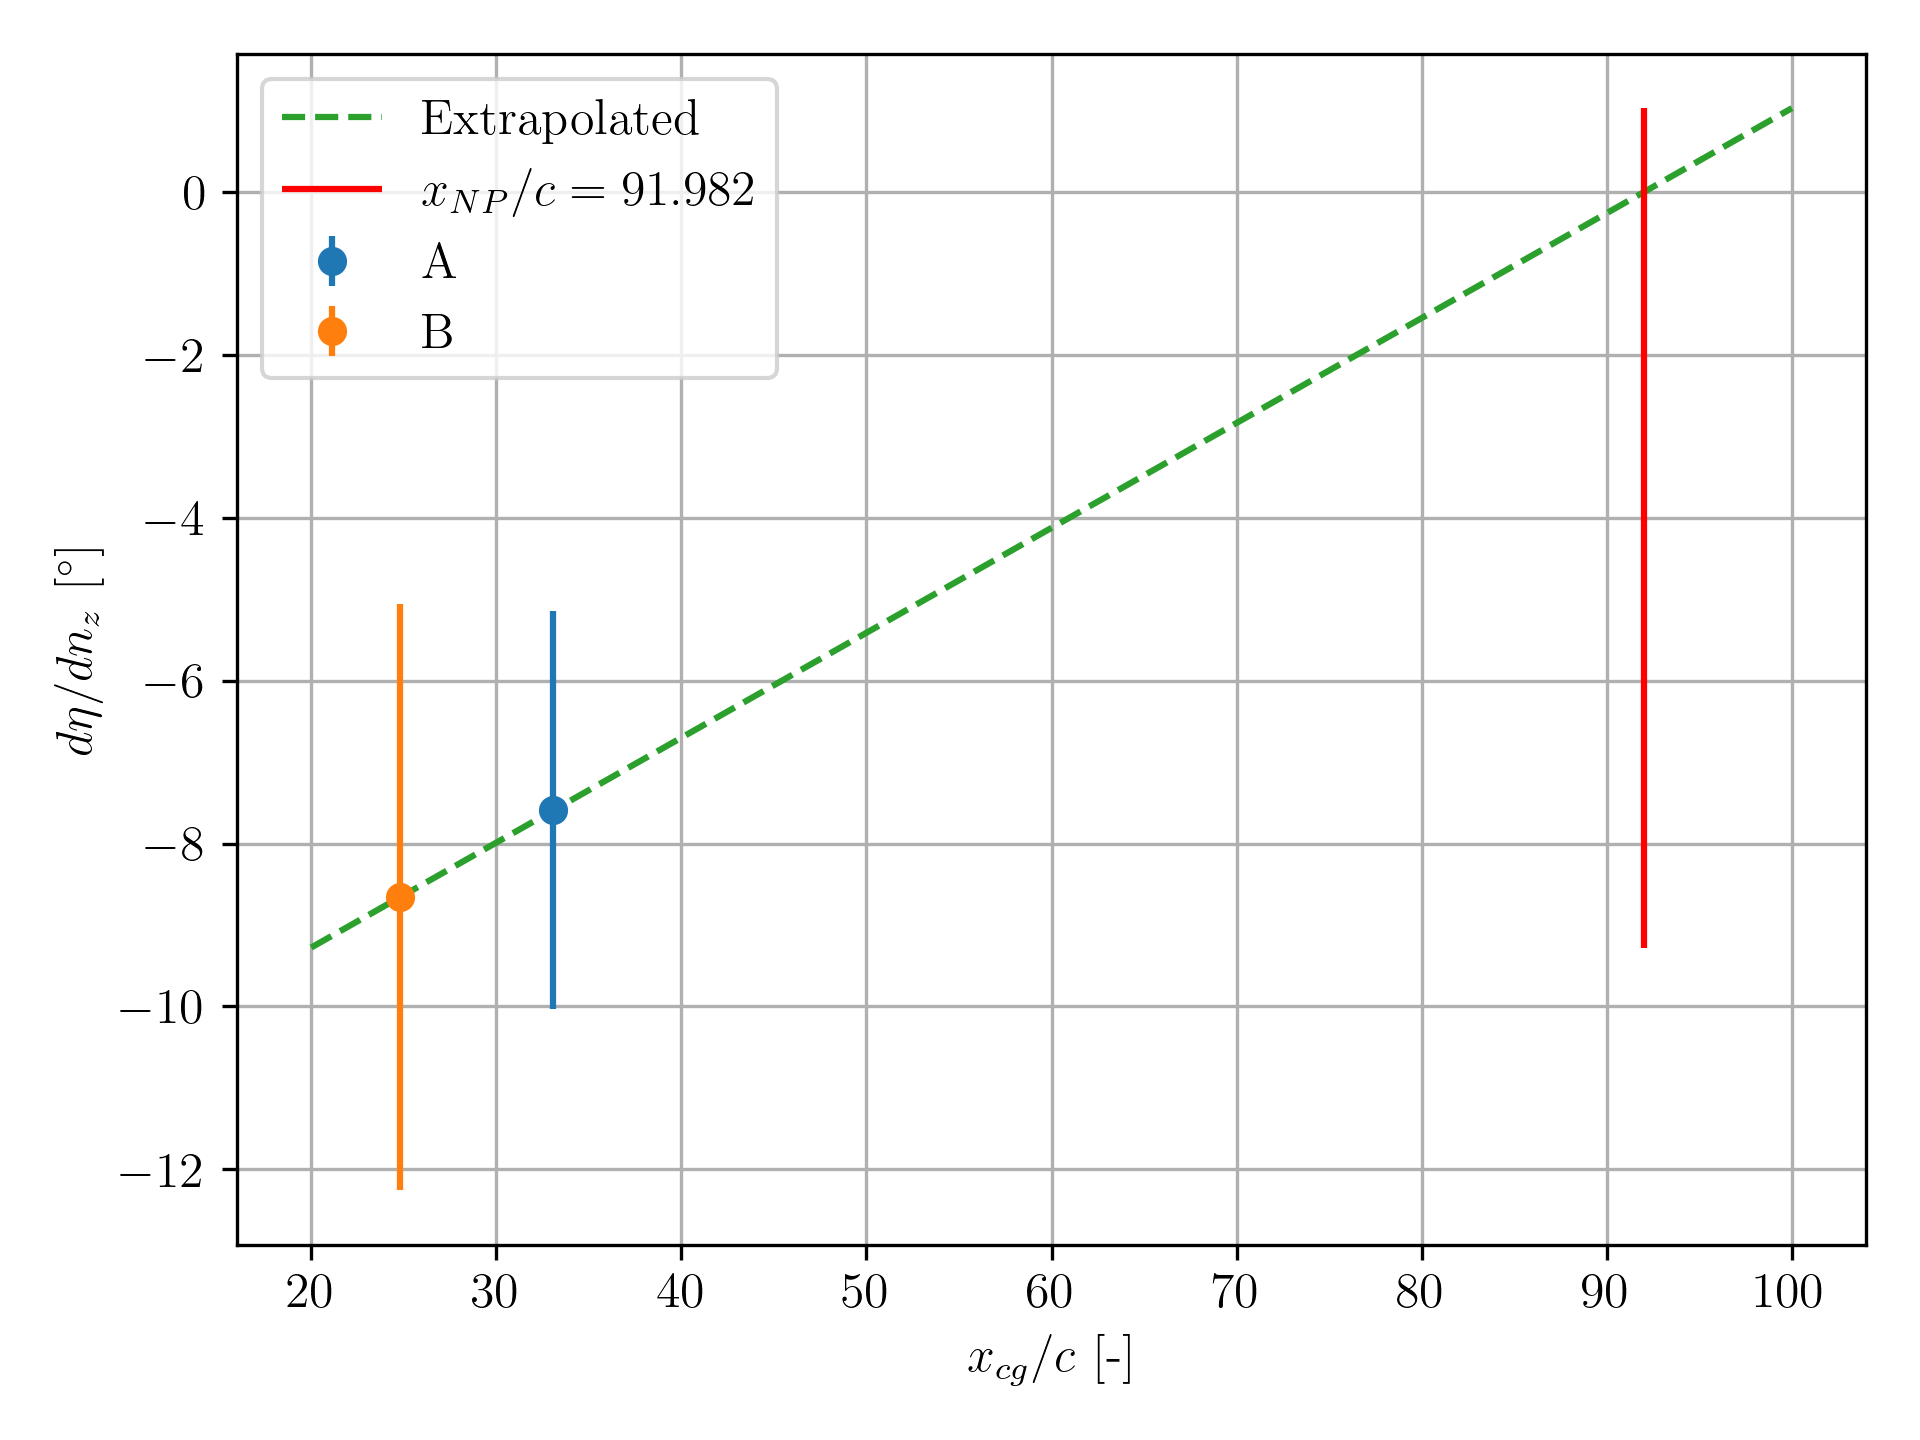
\includegraphics[width=0.8\textwidth]{Manoeuvre_Stability_2.png}
    \caption{}
    \label{fig:Manoeuvre_Stability_2}
\end{figure}
\subsubsection{Stick free manoeuvre point}
\begin{figure}[H]
    \centering
    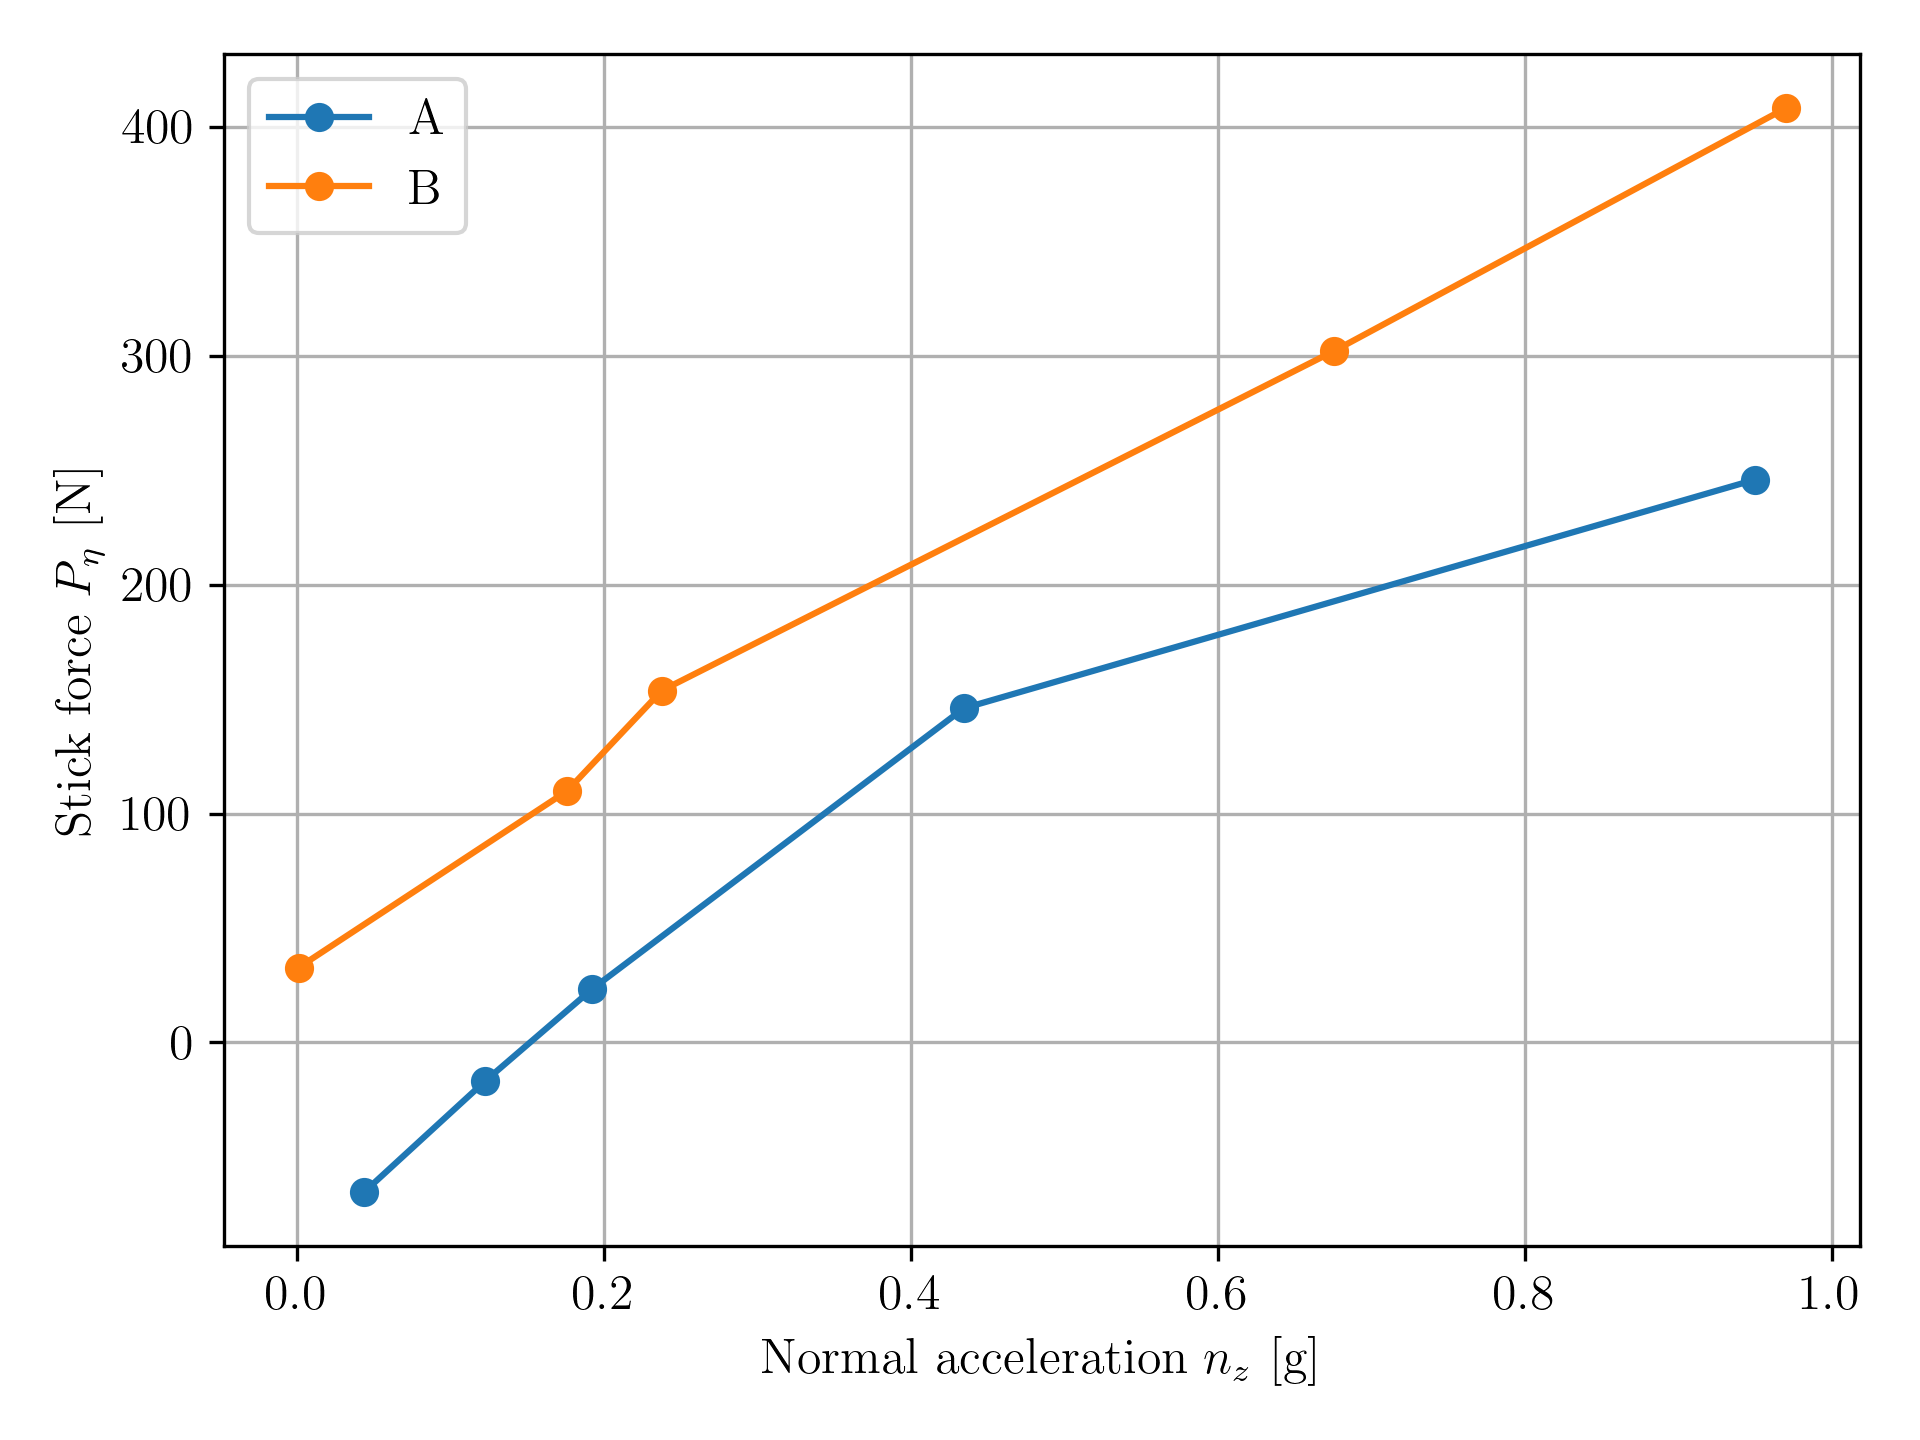
\includegraphics[width=0.8\textwidth]{Manoeuvre_Stability_3.png}
    \caption{}
    \label{fig:Manoeuvre_Stability_3}
\end{figure}
\begin{figure}[H]
    \centering
    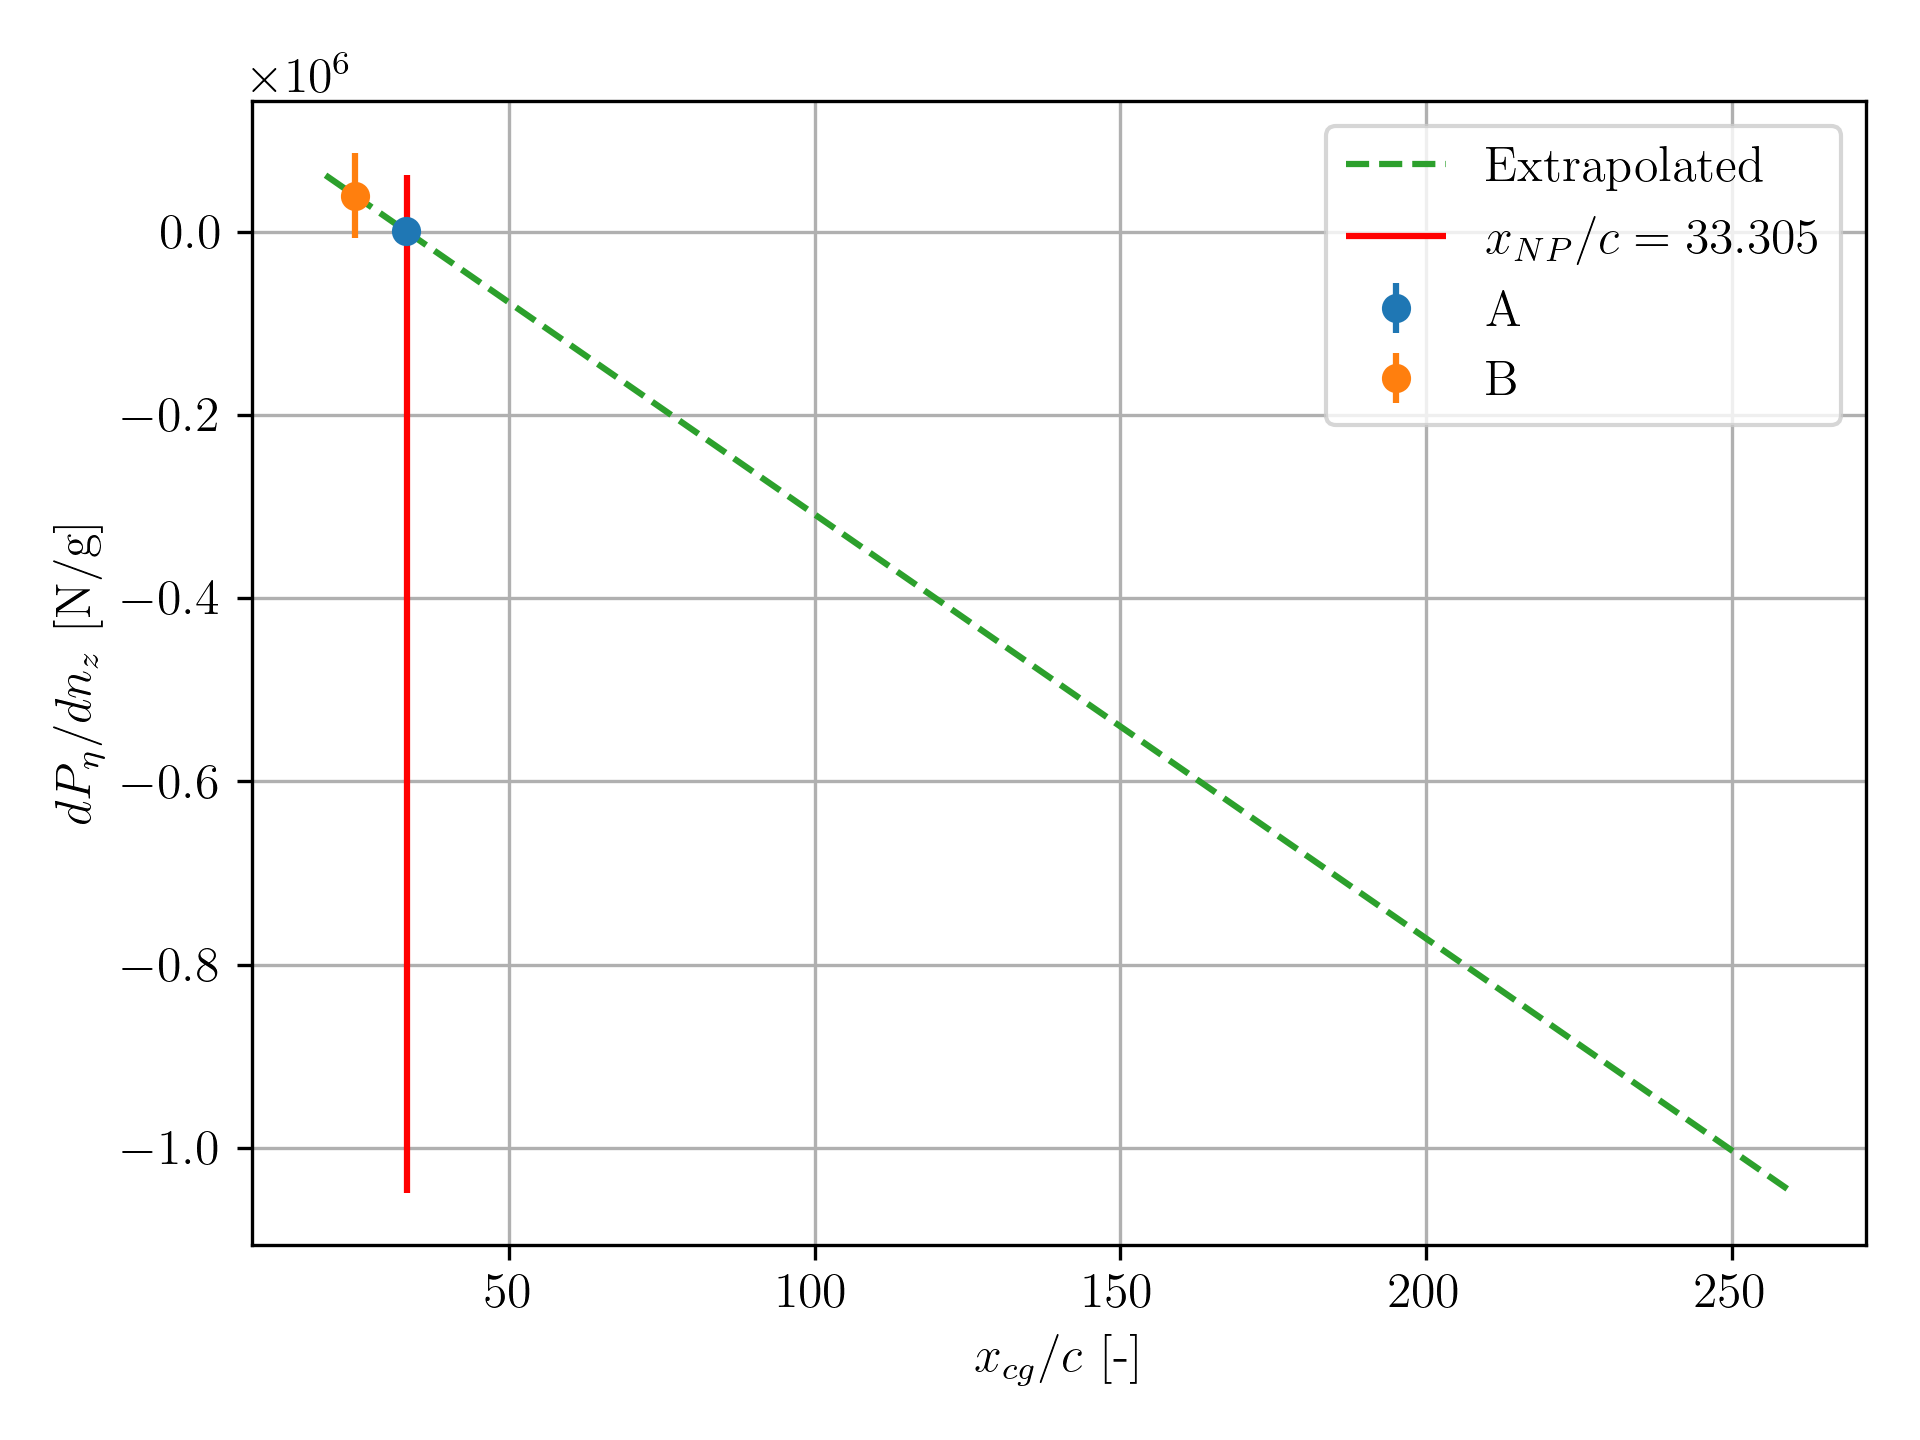
\includegraphics[width=0.8\textwidth]{Manoeuvre_Stability_4.png}
    \caption{}
    \label{fig:Manoeuvre_Stability_4}
\end{figure}

\subsection{Lateral-Directional Static Stability}

\begin{table}[H]
    \centering
    \begin{tabular}{lllll}
        \toprule
        Group A & Aileron angle deg & Roll angle deg & Sideslip deg & Rudder deg \\
        \midrule
        & -1.062 & 0.597 & 0.505 & 0.883 \\
        & -3.431 & 4.001 & 3.284 & 4.497 \\
        & -5.625 & 3.313 & 4.695 & 6.422 \\
        & -7.276 & 4.809 & 5.599 & 8.163 \\
        & 2.867 & -0.958 & -3.175 & -3.353 \\
        & 4.240 & -2.494 & -4.570 & -5.397 \\
        & 5.875 & -4.029 & -5.961 & -7.258 \\
        \bottomrule
        \end{tabular}
\end{table}
\begin{table}{H}
    \centering
        \begin{tabular}{lllll}
        \toprule
        Group B & Aileron angle deg & Roll angle deg & Sideslip deg & Rudder deg \\
        \midrule
        & -0.644 & 0.931 & 0.309 & 0.046 \\
        & 2.172 & -4.042 & -3.299 & -4.176 \\
        & 2.905 & -3.466 & -4.446 & -5.914 \\
        & 4.218 & -5.298 & -5.870 & -7.528 \\
        & -1.758 & 2.847 & 1.788 & 3.012 \\
        & -2.761 & 3.898 & 2.429 & 4.239 \\
        & -3.580 & 4.692 & 3.183 & 5.629 \\
        \bottomrule
        \end{tabular}
\end{table}

\begin{figure}[H]
    \centering
    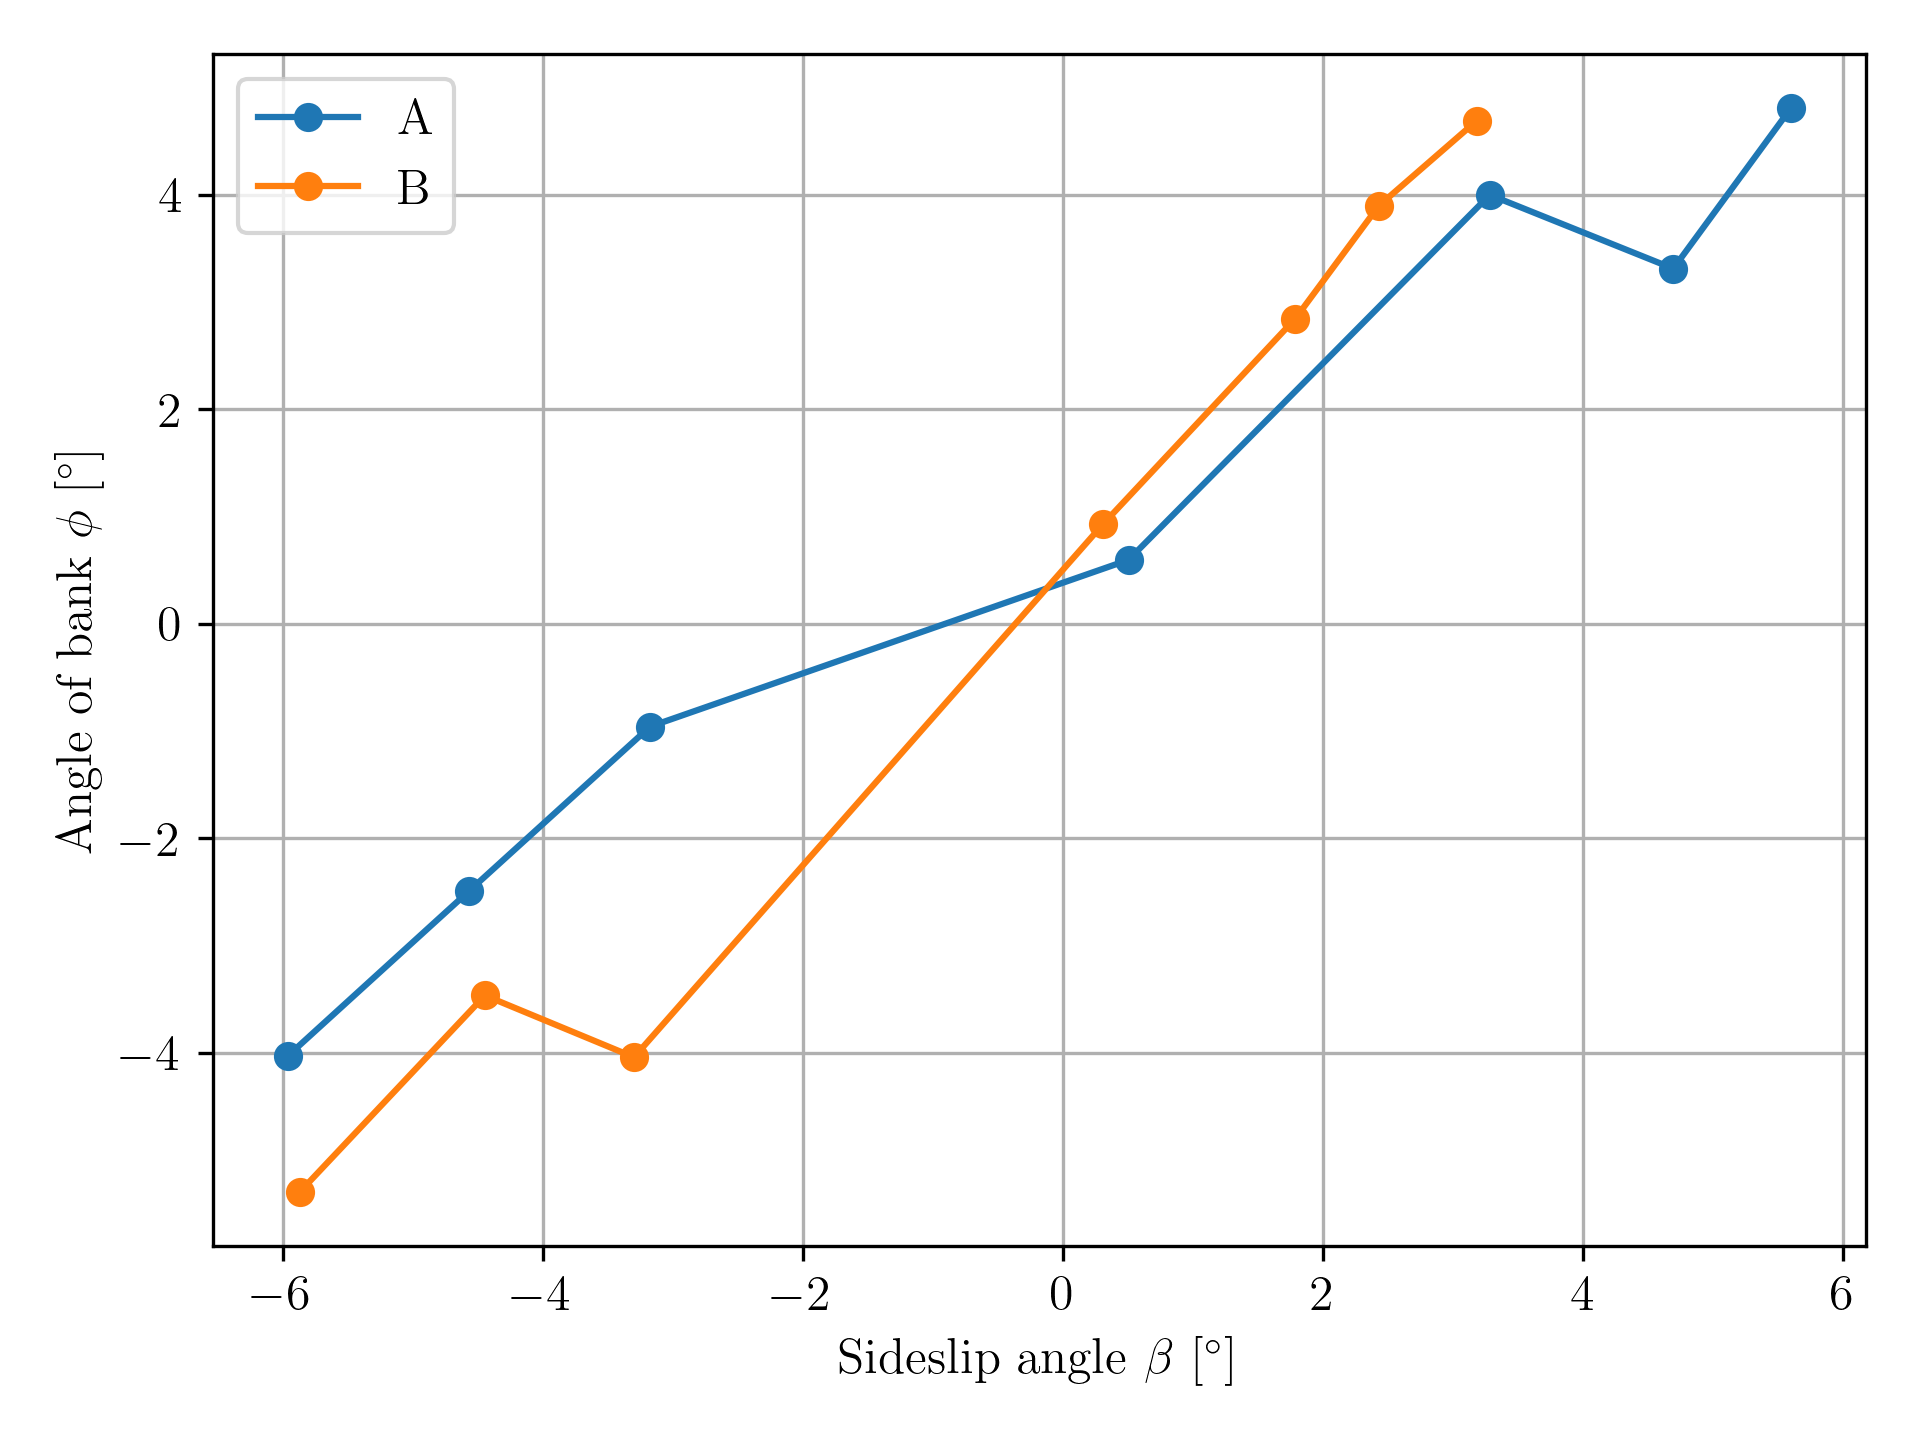
\includegraphics[width=0.8\textwidth]{Lat_Directional_Static_Stability_SHSS_1.png}
    \caption{}
    \label{fig:Lat_Directional_Static_Stability_SHSS_1}
\end{figure}

\subsubsection{Stick fixed lateral directional stability}
\begin{figure}[H]
    \centering
    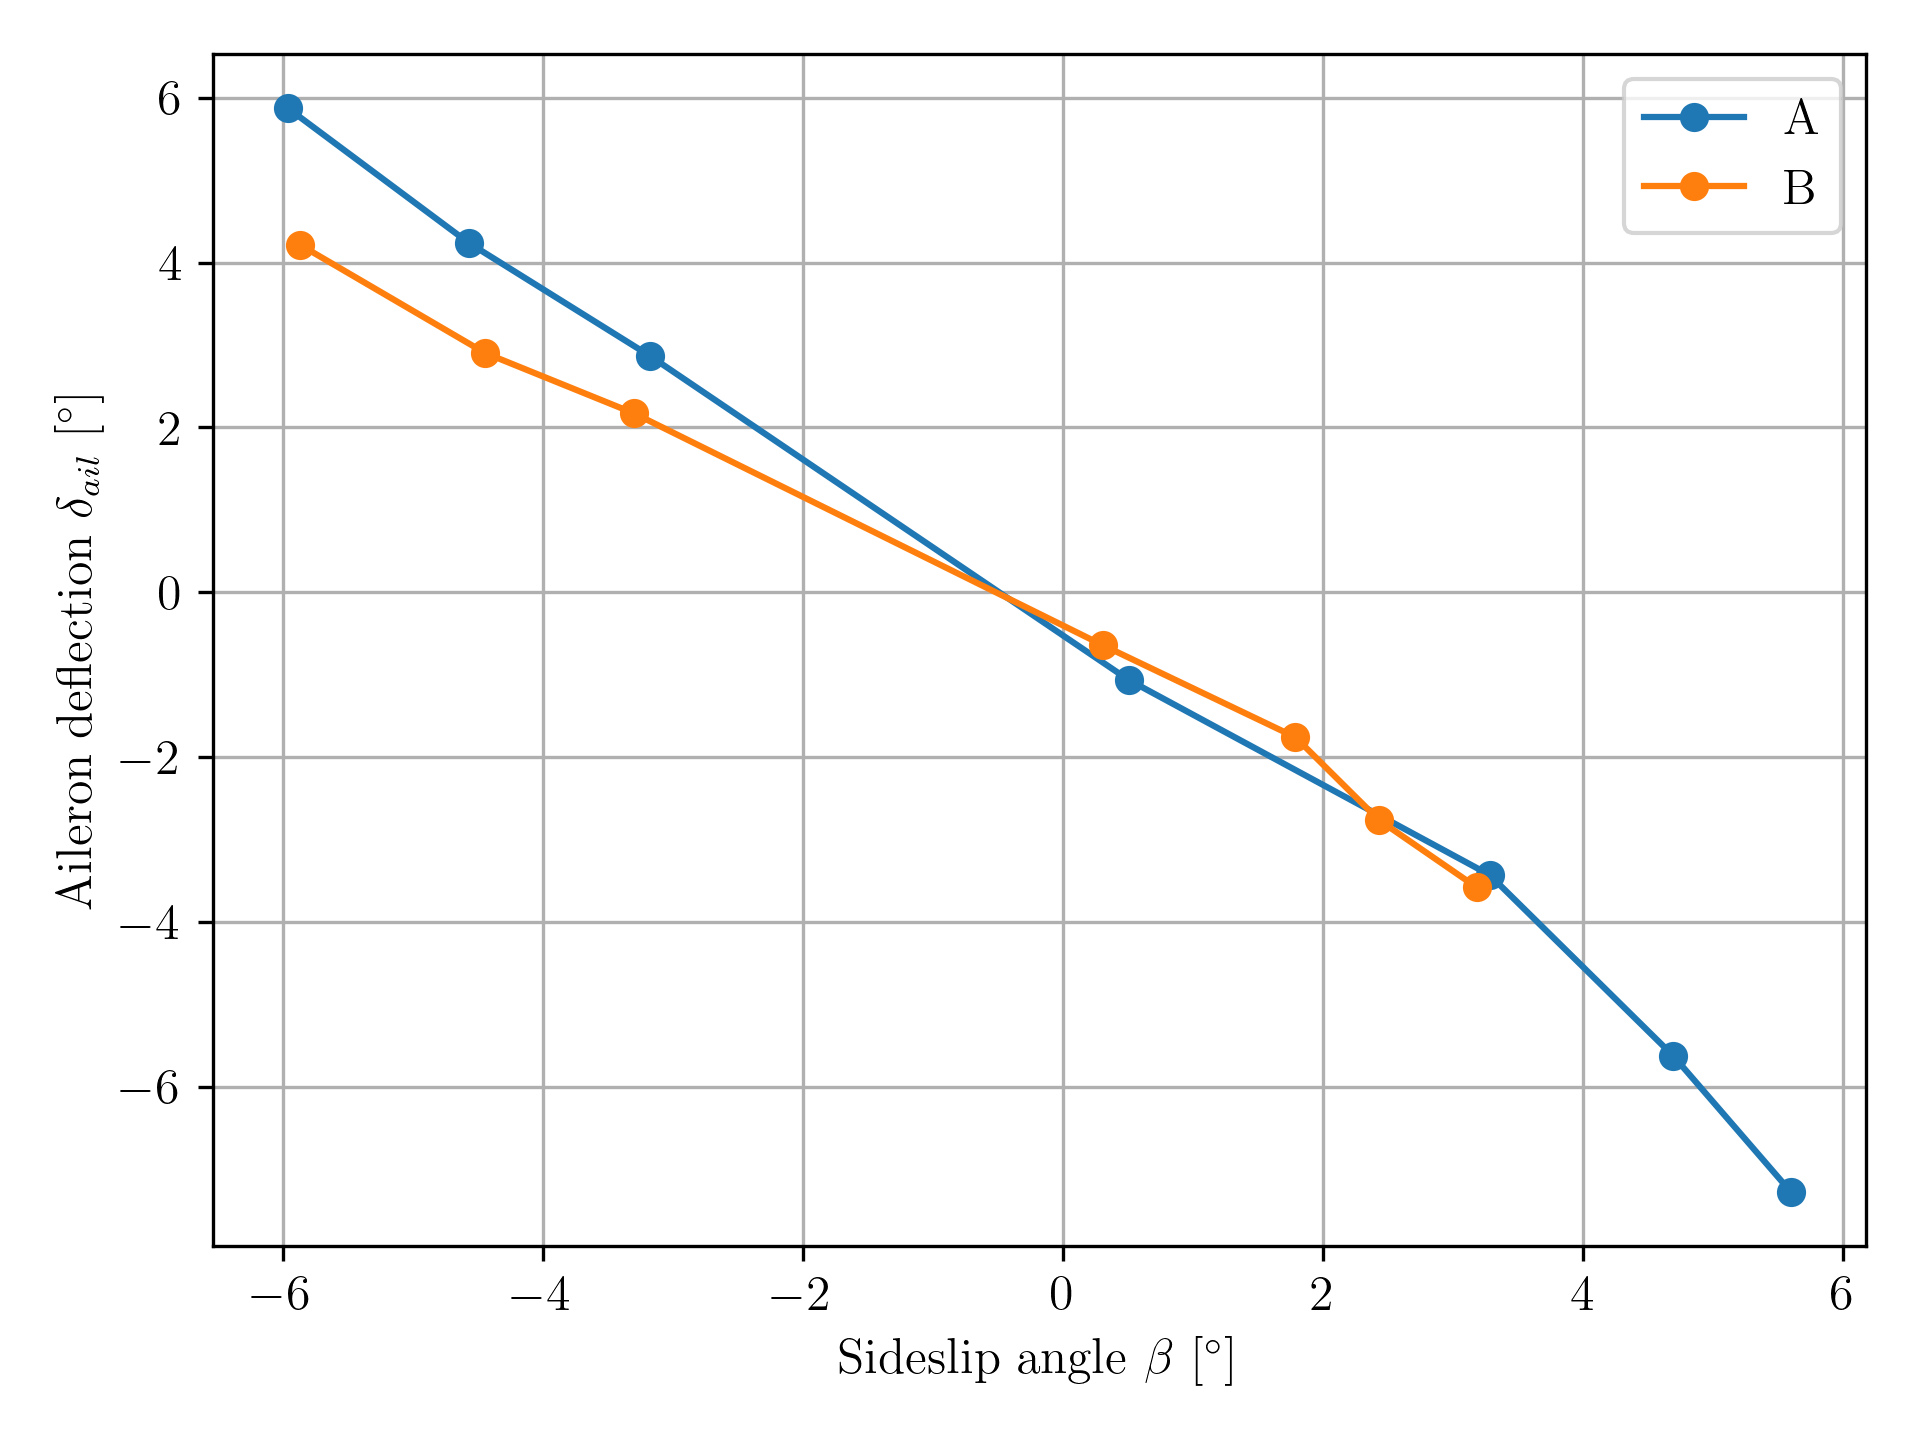
\includegraphics[width=0.8\textwidth]{Lat_Directional_Static_Stability_SHSS_2.png}
    \caption{}
    \label{fig:Lat_Directional_Static_Stability_SHSS_2}
\end{figure}

\begin{figure}[H]
    \centering
    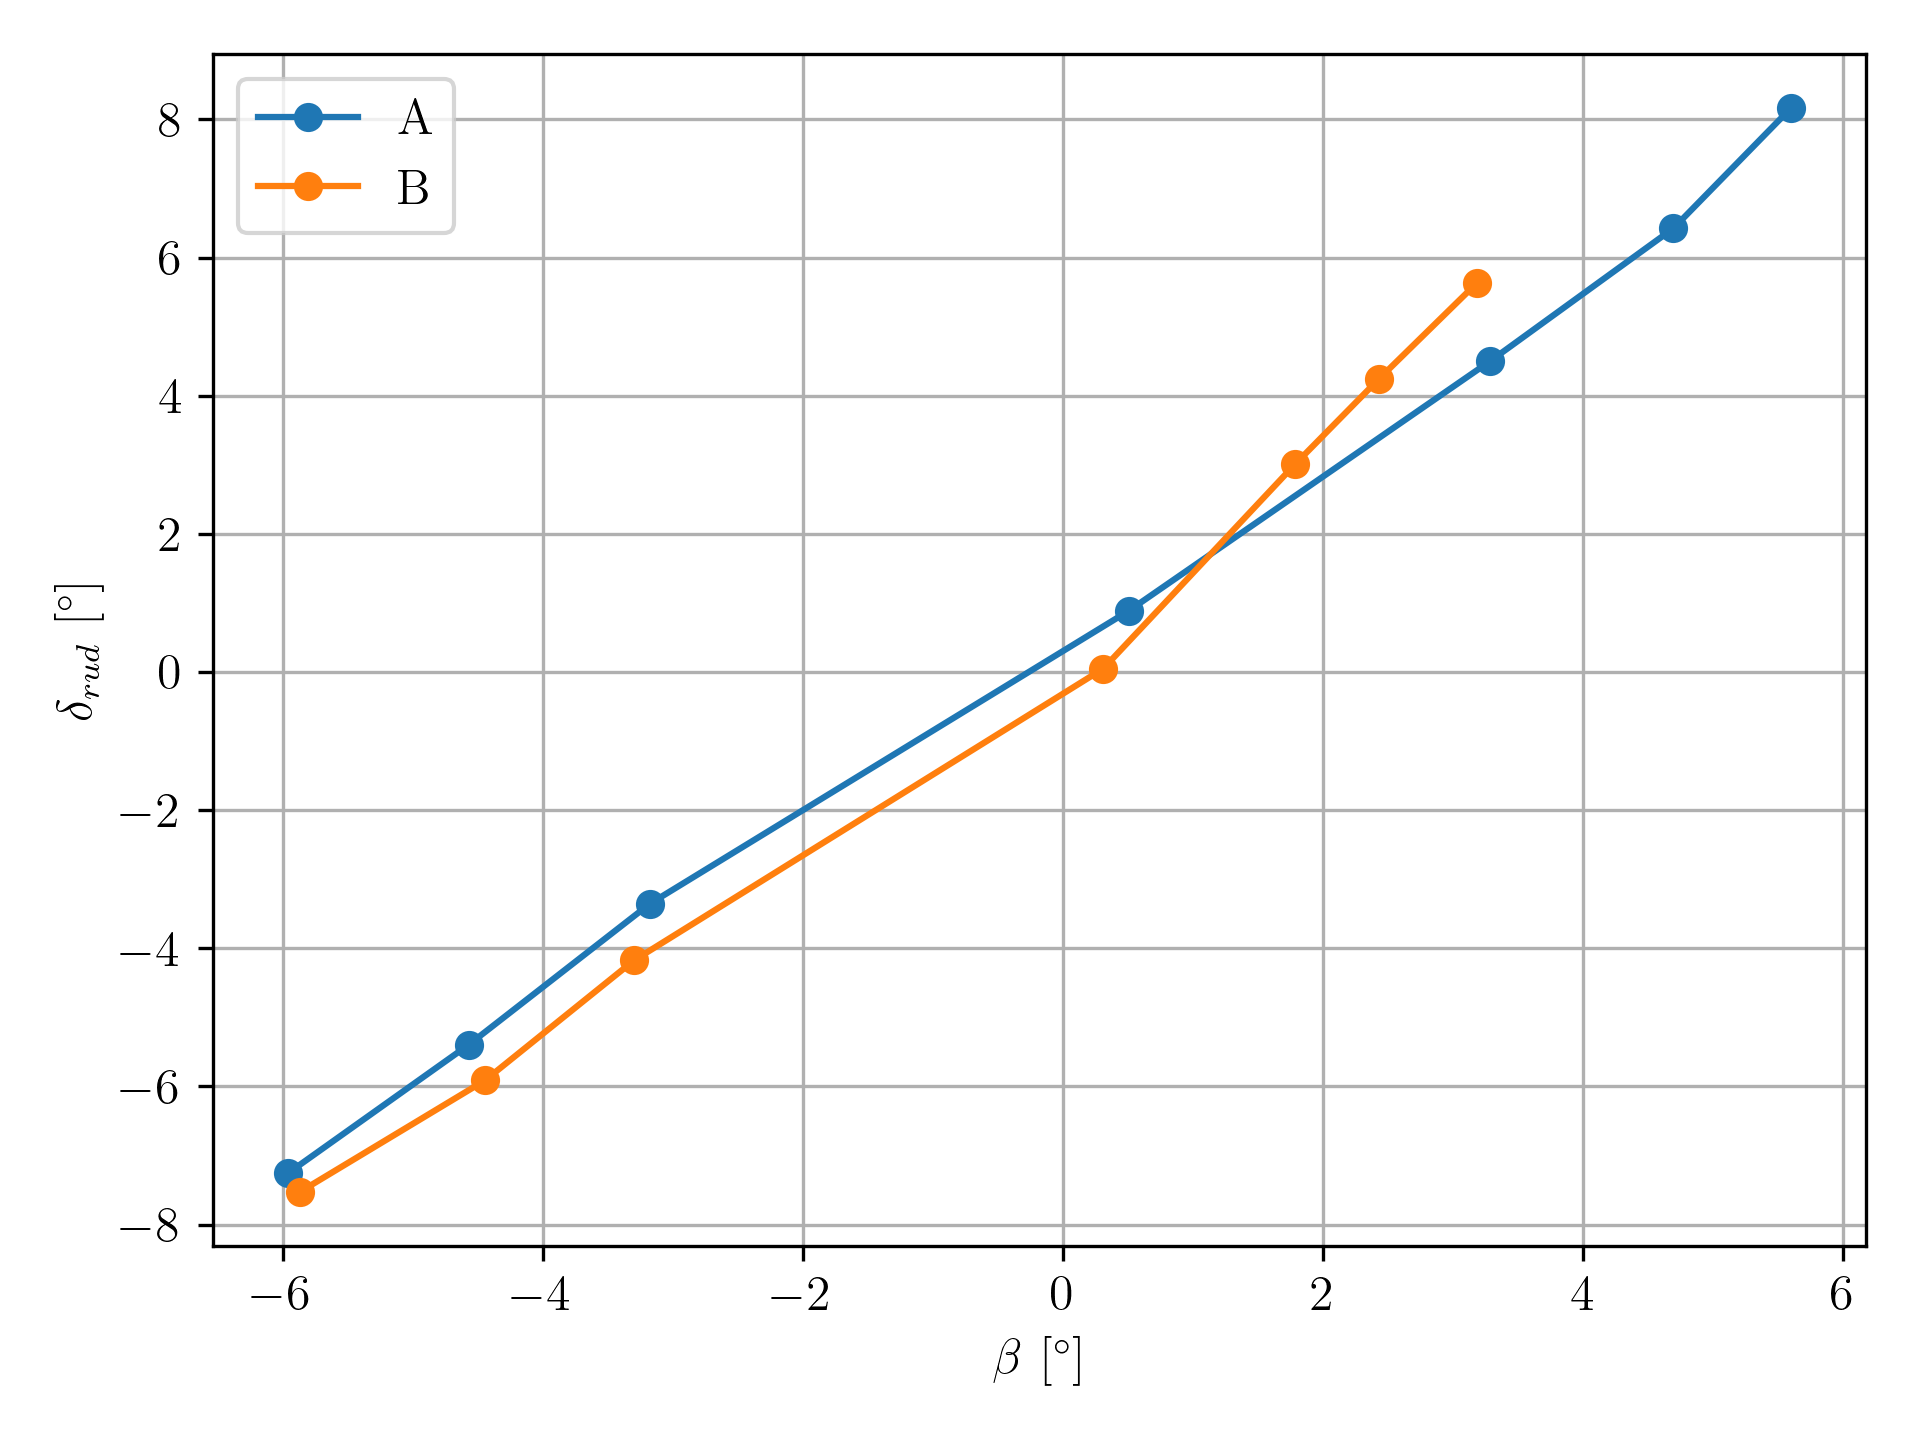
\includegraphics[width=0.8\textwidth]{Lat_Directional_Static_Stability_SHSS_3.png}
    \caption{}
    \label{fig:Lat_Directional_Static_Stability_SHSS_3}
\end{figure}


\begin{thebibliography}{9}

  \bibitem{handout}
  S. Place, A. Cooke
  \emph{Flight Experimental Methods: Course Handbook}
  Cranfield University,

\end{thebibliography}

\end{document}

